\section{Iteration 6: Decomposition of the Scheduler for Anomaly Detection}
\label{add:it6}

\subsection{Step 1: Identify candidate drivers}
\label{add:it6/drivers}

\npar This iteration is driven by P2': Anomaly detection. The description states
that the load should be balanced ower multiple instances of each subsystem.

\subsection{Step 2: Choose design concepts}
\label{add:it6/concepts}

\subsubsection{Tactics}
\label{add:it6/tactics}

\npar Because anomaly detection algorithms are complicated calculations on large
datasets, it is inherently slow. One simply cannot wait until this process is
completed. Therefore, parallellism is introduced as a tactic. 

\npar This tactic calls for multiple instances but there will not be an infinite
number of resources. Some resource arbitration should be put in place to make
the use of resources efficient. 

\subsubsection{Design Patterns}
\label{add:it6/patterns}

\paragraph{Resource Pool}

\npar The resource pool design pattern \citep[see][p.~503]{Buschmann:07} can be
used to efficiently manage the instances for anomaly detection. Every time an
anomaly request comes in, an instance is removed from the pool and assigned to
that request. When the anomaly detection algorithm has ended, the resource is
placed back in the pool. 

\paragraph{Replicated Component Group}

\npar Running all instances on a single machine is not the best idea. If that
machine goes down, there is no way to detect anomalies. A better approach is to
distribute multiple instances across multiple nodes. As with database
replication, the replicated component group design pattern
\citep[see][p.~326]{Buschmann:07} can be used.

\paragraph{Business Delegate}

\npar To make the location of the instances transparant, a business delegate
design pattern \citep[see][p.~292]{Buschmann:07} can be used, as is done in
iteration 4 (see \ref{add:it4}) for the measurements storage replication.

\subsection{Step 3: Instantiate architectural elements and allocate responsibilities}
\label{add:it6/elements}

\npar For every incoming command (ADCommand), the front end (ADFrontEnd) will
remove an anomaly detection instance (ADInstance) from the resource pool
(ADInstancePool). This instance will handle the anomaly detection for that
command and will return the result in a callback to the front end. The front end
will then handle the result and if necessary dispatch the Notification Unit.
After this is done, the instance is placed back in the pool.

\npar An overview of the instantiated child components of the Anomaly Detection
Unit is shown in \ref{fig:it6/elements}.

\begin{figure}[H]
	\begin{centering}
		% TODO Figure
		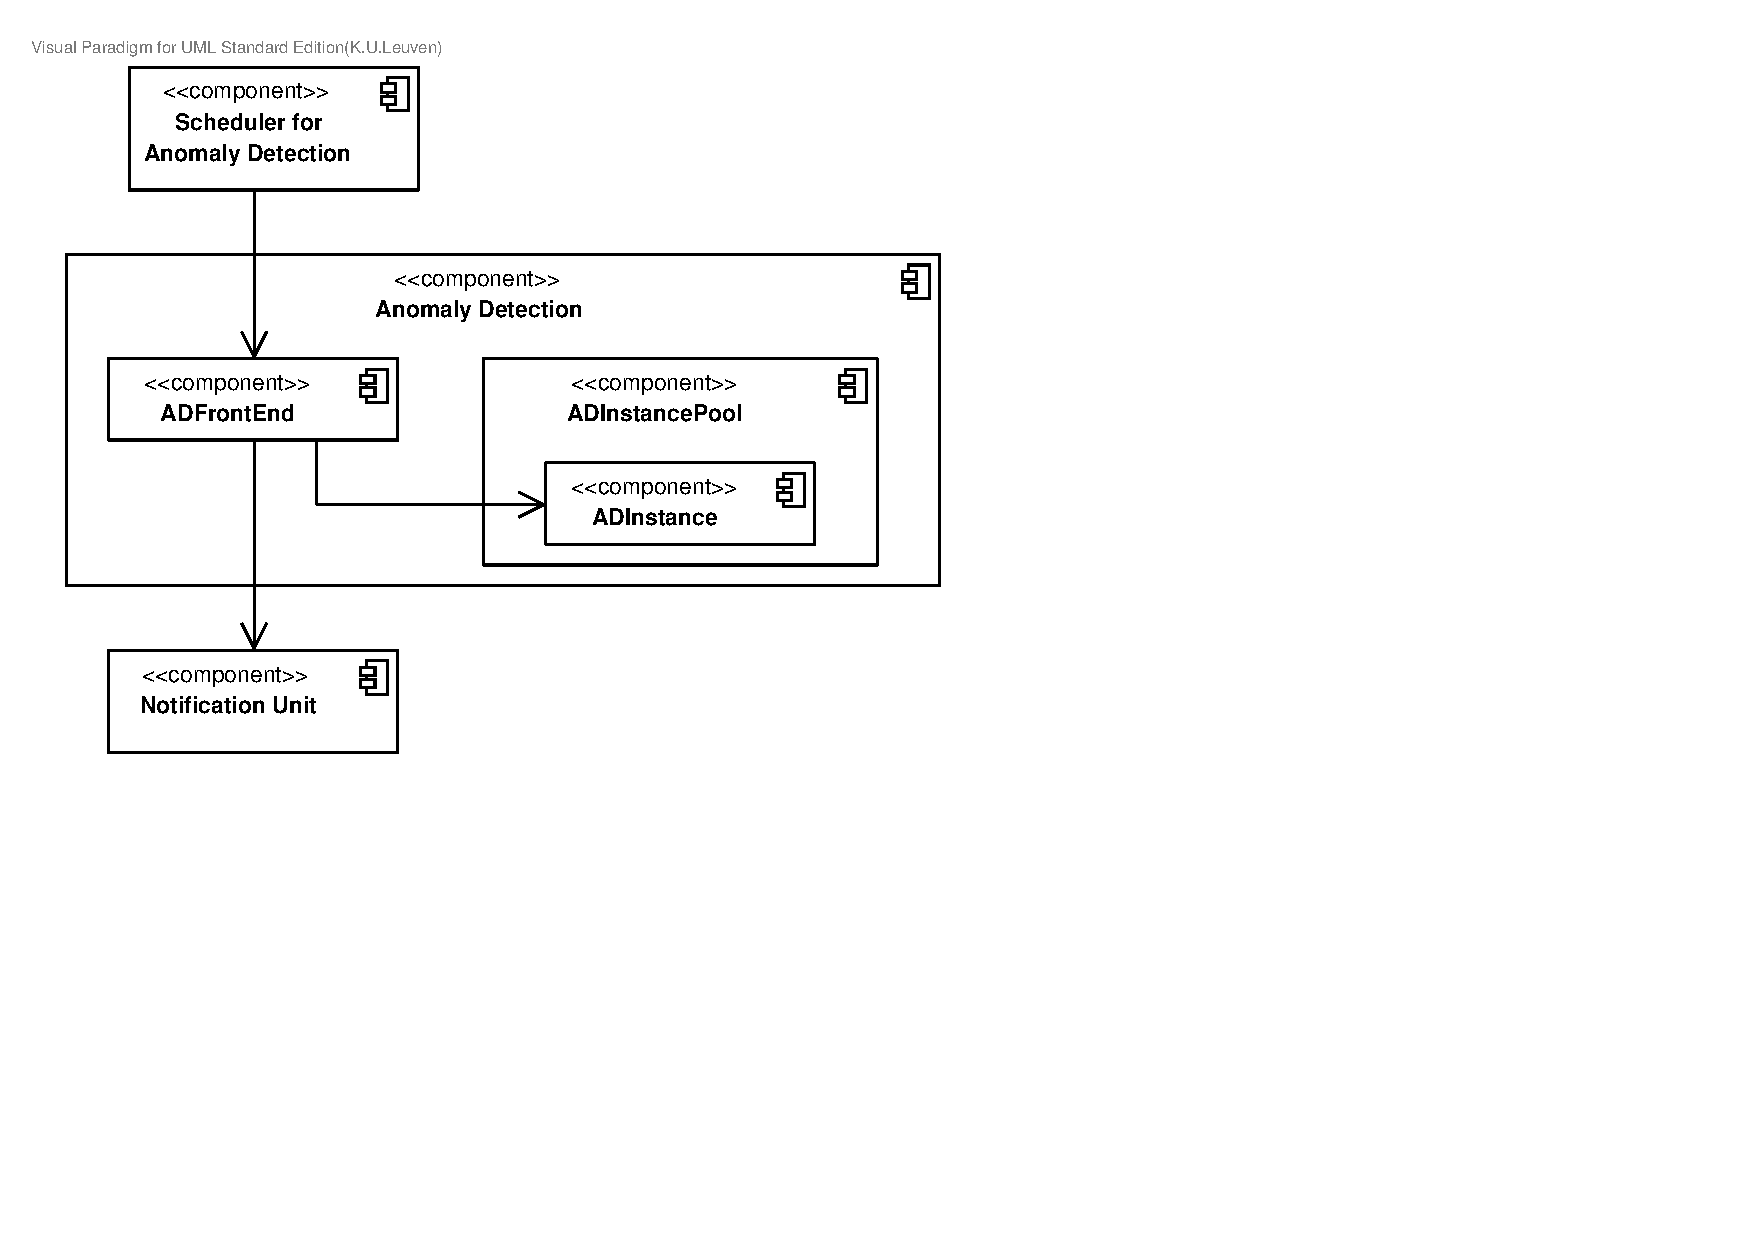
\includegraphics[width=\textwidth]{figs/add-it6-elements.pdf}
		\caption{Overview of all instantiated child elements in the Anomaly
		Detection Unit}
		\label{fig:it6/elements}
	\end{centering}
\end{figure}

\subsection{Step 4: Define interfaces for instantiated elements}
\label{add:it6/interfaces}

\subsubsection{AnomalyDetectionAPI}

\npar The ADFrontEnd exposes an interface \interface{AnomalyDetectionAPI}, which
accepts ADCommands with the \method{execute(QueryCommand)} method.

\subsubsection{ADInstancePoolAPI}

\npar The ADFrontEnd must remove an instance from the pool and uses the
\method{remove()} method from \interface{ADInstancePoolAPI}, provided by
ADInstancePool, for this purpose.

\npar When the calculations are done, the ADFrontEnd adds the instance back to
the pool using the \method{add(ADInstance)} method.

\subsubsection{ADInstanceAPI}

\npar To actually run an anomaly detection algorithm, the mehod
\method{execute(ADCommand, Callback)} from the \interface{ADInstanceAPI}
interface is used. This is an asynchronous method call. It will return
immediately and return the results back to the front end whenever it is ready.
A Callback object is provided for this purpose. 

\npar On overview of all the components and their interfaces is shown in figure
\ref{fig:it6/interfaces}.

\begin{figure}[H]
	\begin{centering}
		% TODO Figure
		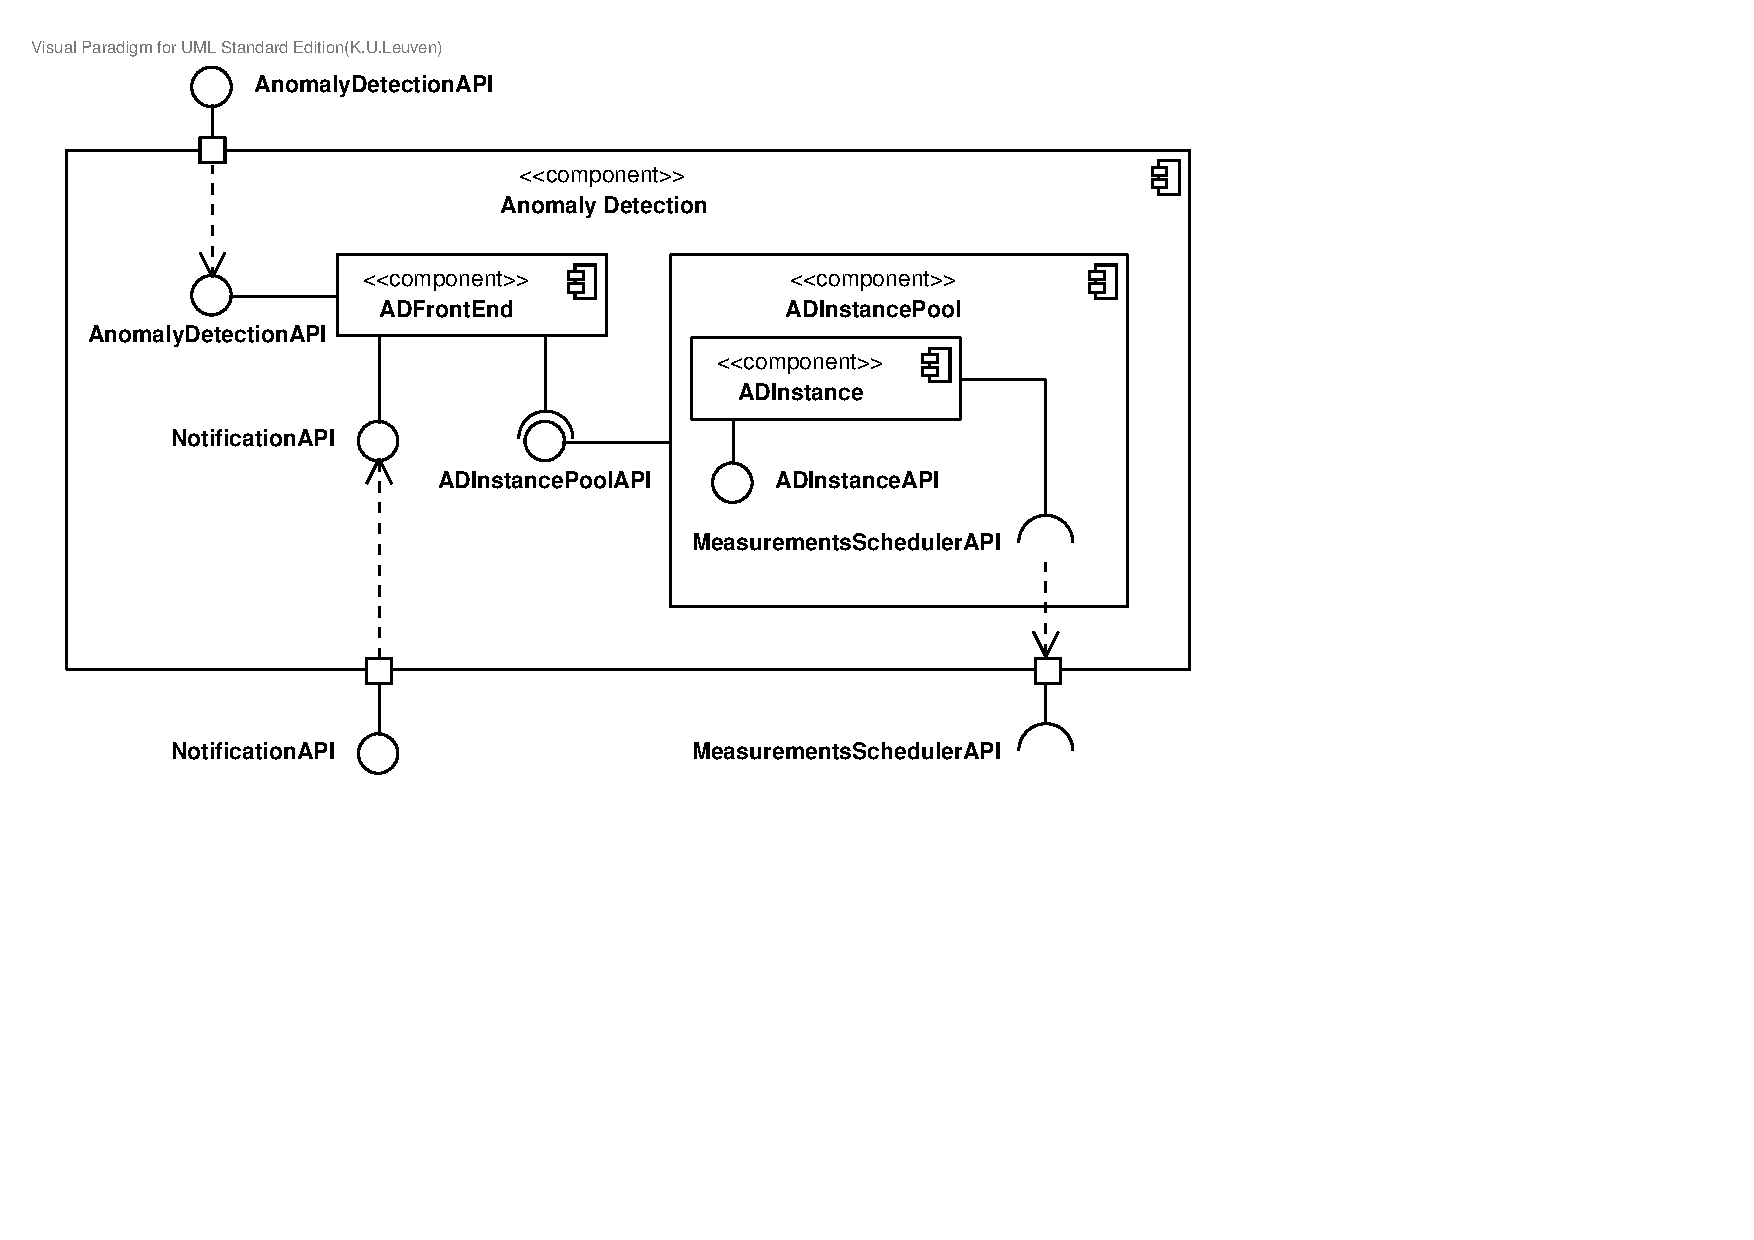
\includegraphics[width=\textwidth]{figs/add-it6-interfaces.pdf}
		\caption{Overview of the interfaces and components in the Anomaly Detection
		Unit}
		\label{fig:it6/interfaces}
	\end{centering}
\end{figure}

\subsection{Step 5: Verify and refine}
\label{add:it6/verification}

\npar The quality attribute P2' (introduce parallellism) is resolved in this
iteration. The actual anomaly detection (UC10) is delegated to ADInstance.
